\chapter{Introduction}

Forests are a crucial part of the global ecosystem, both environmentally and economically.
They cover a third of the land area, contain over 80\% of terrestrial biodiversity, and somewhere around one-third of humanity depends on forests and forest products for their livelihoods \cite{aertsForestRestorationBiodiversity2011,StateWorldsForests2020}.
Forests are an essential renewable natural resource and a huge, dynamic part of the global carbon cycle.
Responsible management of forests allows using the resources efficiently and sustainably, preserving the biodiversity, and regulating atmospheric $CO_2$, which is becoming especially important as the anthropogenic climate change is ongoing and accelerating \cite{faheyForestCarbonStorage2010,forsterIndicatorsGlobalClimate2024}.
This drives the need for accurate, detailed, up-to-date information about various forest attributes such as distributions of species, heights, ages of trees, timber volume and above ground biomass estimates, and others.

The traditional manual forest inventories are extremely labor-intensive and time-consuming, which makes them infeasible to cover extensive areas with sufficient detail, speed, and frequency \cite{burleyEncyclopediaForestSciences2004}.


\todo[inline]{TODO: complete chapter}

\section{Thesis Structure}
The diagram in \autoref{fig:thesis-structure} illustrates the flow of information through the structure of the thesis.

\begin{figure}[htb!]
\centering 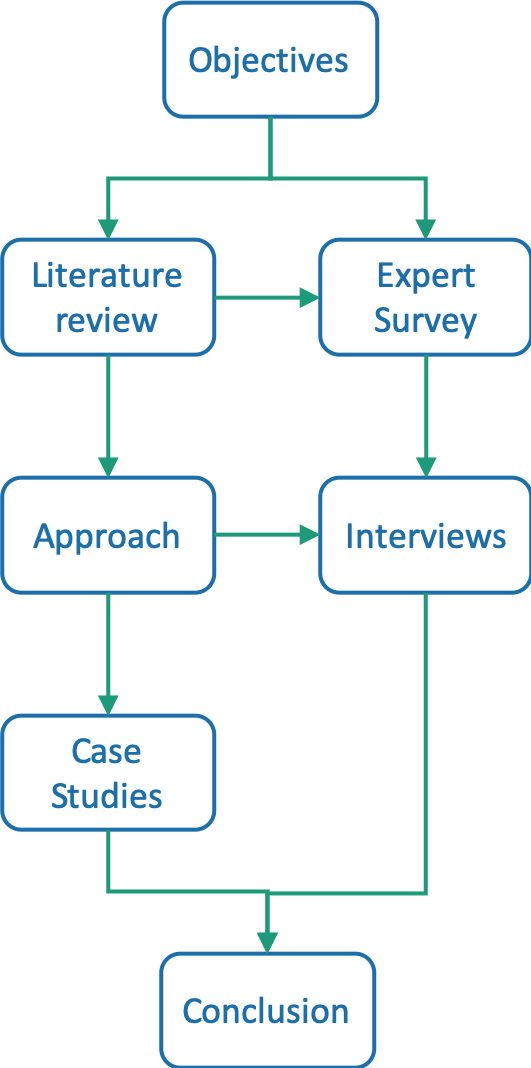
\includegraphics[width=0.5\textwidth]{graphics/thesis-structure}
\caption{Thesis structure}
\label{fig:thesis-structure}
\end{figure}

\begin{description}
    \item[\Autoref{cap:background} - Background]
Here's the literature review.

    \item[\Autoref{cap:thesis_objectives} - Thesis Objectives]
We define the objectives of our work.

...

    \item[\Autoref{cap:conclusion} - Conclusion]
In the last chapter, we discuss our results obtained ...

\end{description}